\documentclass[tikz]{standalone}

\usepackage{tikz}
\usetikzlibrary{decorations}
\usetikzlibrary{decorations.pathreplacing, intersections}
\usepackage{pgfplots}
\usetikzlibrary{calc,positioning}
\pgfplotsset{compat=newest, scale only axis, width = 10cm}

% ---------------------------------------------------------------------
% Coordinate extraction
% #1: node name
% #2: output macro name: x coordinate
% #3: output macro name: y coordinate
\newcommand{\Getxycoords}[3]{%
    \pgfplotsextra{%
        % using `\pgfplotspointgetcoordinates' stores the (axis)
        % coordinates in `data point' which then can be called by
        % `\pgfkeysvalueof' or `\pgfkeysgetvalue'
        \pgfplotspointgetcoordinates{(#1)}%
        % `\global' (a TeX macro and not a TikZ/PGFPlots one) allows to
        % store the values globally
         \global\pgfkeysgetvalue{/data point/x}{#2}%
         \global\pgfkeysgetvalue{/data point/y}{#3}%
     }%
}
% ---------------------------------------------------------------------

% Create fake \onslide and other commands for standalone picture
\usepackage{xparse}
\NewDocumentCommand{\onslide}{s t+ d<>}{}
\NewDocumentCommand{\only}{d<>}{}
\NewDocumentCommand{\uncover}{d<>}{}
\NewDocumentCommand{\visible}{d<>}{}
\NewDocumentCommand{\invisible}{d<>}{}

\begin{document}

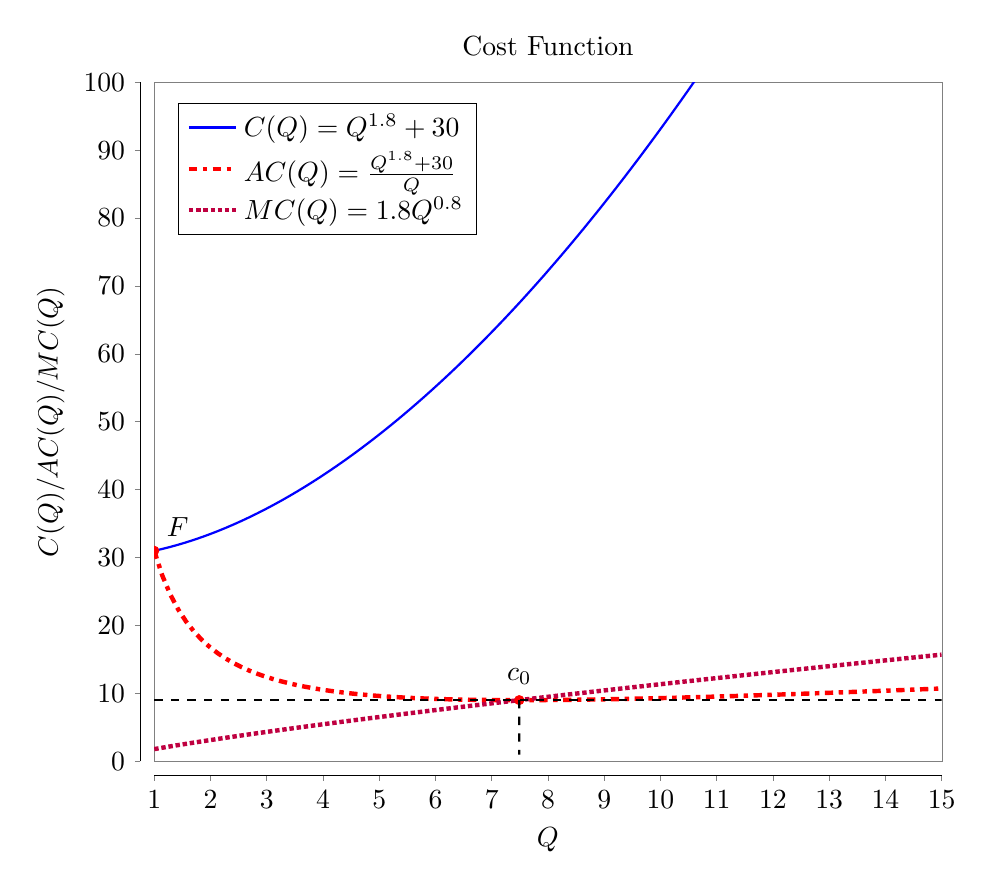
\begin{tikzpicture}


\begin{axis}[
    xmin = 1,
    xmax = 15,
    ymin = 0,
    ymax = 100,
    xlabel = {$Q$},
    ylabel = {$C(Q)/AC(Q)/MC(Q)$},
    sciclean/.style={axis lines=left,
        axis x line shift=0.5em,
        axis y line shift=0.5em,
        axis line style={-,very thin},
        axis background/.style={draw,ultra thin,gray},
        tick align=outside,
        major tick length=2pt},
    xtick distance=1,
    ytick distance=10,
    title = {Cost Function},
    domain = 1:15,
    legend cell align = left,
    legend pos = north west,
    sciclean]

    \addplot[name path = C, thick, color = blue, samples = 100] {x^1.8 + 30};
    \addlegendentry{$ C(Q) = Q^{1.8} + 30$}
    \path[name path=Y]  (1,0) -- (1,100);
    \path[name intersections={of = C and Y, by=y0}]
        node[fill=red,circle,inner sep=1.3pt, label={60:$F$}] at (y0)  {};
    \addplot[name path = AC, ultra thick, color = red, dashdotted, samples = 100] {(x^1.8 + 30) / x};
    \addlegendentry{$ AC(Q) = \frac{Q^{1.8} + 30}{Q} $}
    \addplot[name path = MC, ultra thick, color = purple, densely dotted, samples = 100] {1.8*x^0.8};
    \addlegendentry{$ MC(Q) = 1.8 Q^{0.8} $}
    \path[name intersections={of = AC and MC, by=c0}];
    \node[fill=red,circle,inner sep=1.3pt, label={[align=left] 90:$c_{0}$ }] at (c0)  {};
    \Getxycoords{c0}{\xC}{\yC}
    \draw[dashed, thick] (1, \yC) -- (20, \yC);
    \draw[dashed, thick] (c0) -- (\xC, 1);

\end{axis}

    % We could control parts of figure only shown in beamer or vice versa.
    % \ifstandalone
    %     \node[below=1cm of mid] {Only Shown in Standalone Figure};
    % \else
    %     \node[below=1cm of mid] {Only Shown in Beamer};
    % \fi
\end{tikzpicture}

\end{document}
